%%%%%%%%%%%%%%%%%%%%%%%%%%%%%%%%%%%%%%%%%%%%%%%%%%%%%%%%%%%%%%%%%%%%%%%%%%%%%%%%%%%%%%%%%%%%%%%%
%
% CS484 Written Question Template
%
% Acknowledgements:
% The original code is written by Prof. James Tompkin (james_tompkin@brown.edu).
% The second version is revised by Prof. Min H. Kim (minhkim@kaist.ac.kr).
%
% This is a LaTeX document. LaTeX is a markup language for producing 
% documents. Your task is to fill out this document, then to compile 
% it into a PDF document. 
%
% 
% TO COMPILE:
% > pdflatex thisfile.tex
%
% If you do not have LaTeX and need a LaTeX distribution:
% - Personal laptops (all common OS): www.latex-project.org/get/
% - We recommend latex compiler miktex (https://miktex.org/) for windows,
%   macTex (http://www.tug.org/mactex/) for macOS users.
%   And TeXstudio(http://www.texstudio.org/) for latex editor.
%   You should install both compiler and editor for editing latex.
%   The another option is Overleaf (https://www.overleaf.com/) which is 
%   an online latex editor.
%
% If you need help with LaTeX, please come to office hours. 
% Or, there is plenty of help online:
% https://en.wikibooks.org/wiki/LaTeX
%
% Good luck!
% Min and the CS484 staff
%
%%%%%%%%%%%%%%%%%%%%%%%%%%%%%%%%%%%%%%%%%%%%%%%%%%%%%%%%%%%%%%%%%%%%%%%%%%%%%%%%%%%%%%%%%%%%%%%%
%
% How to include two graphics on the same line:
% 
% \includegraphics[width=0.49\linewidth]{yourgraphic1.png}
% \includegraphics[width=0.49\linewidth]{yourgraphic2.png}
%
% How to include equations:
%
% \begin{equation}
% y = mx+c
% \end{equation}
% 
%%%%%%%%%%%%%%%%%%%%%%%%%%%%%%%%%%%%%%%%%%%%%%%%%%%%%%%%%%%%%%%%%%%%%%%%%%%%%%%%%%%%%%%%%%%%%%%%

\documentclass[11pt]{article}
\usepackage[english]{babel}
\usepackage[utf8]{inputenc}
\usepackage[colorlinks = true,
            linkcolor = blue,
            urlcolor  = blue]{hyperref}
\usepackage[a4paper,margin=1.5in]{geometry}
\usepackage{stackengine,graphicx,subfigure}
\usepackage{fancyhdr}
\setlength{\headheight}{15pt}
\usepackage{microtype}
\usepackage{times}

% From https://ctan.org/pkg/matlab-prettifier
\usepackage[numbered,framed]{matlab-prettifier}

\frenchspacing
\setlength{\parindent}{0cm} % Default is 15pt.
\setlength{\parskip}{0.3cm plus1mm minus1mm}

\pagestyle{fancy}
\fancyhf{}
\lhead{Homework 4 Questions}
\rhead{CS484}
\rfoot{\thepage}

\date{}

\title{\vspace{-1.5cm}Homework 4 Questions}


\begin{document}
\maketitle
\vspace{-3cm}
\thispagestyle{fancy}

\section*{Instructions}
\begin{itemize}
  \item 4 questions.
  \item Write code where appropriate.
  \item Feel free to include images or equations.
  \item Please make this document anonymous.
  \item \textbf{Please use only the space provided and keep the page breaks.} Please do not make new pages, nor remove pages. The document is a template to help grading. If you need extra space, please use and refer to new pages at the end of the document.
\end{itemize}

\section*{Questions}

\paragraph{Q1:} Given a linear classifier, how might we handle data that are not linearly separable? How does the \emph{kernel trick} help in these cases? (See course slides in supervised learning, plus your own research.)

%%%%%%%%%%%%%%%%%%%%%%%%%%%%%%%%%%%
\paragraph{A1:} 
When we use linear classifier, we can see data that are not linearly separable. Then, we can separate them in a way that increases the dimension. A prime example is kernel trick.

\begin{figure}[!h]
    \centering
    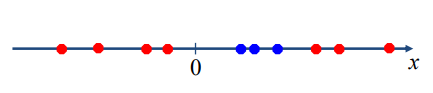
\includegraphics[width=8cm]{q1_1.png}
    \caption{before kernel}
    \label{fig:Question1}
\end{figure}
In this case, we can separate them.

\begin{figure}[!h]
    \centering
    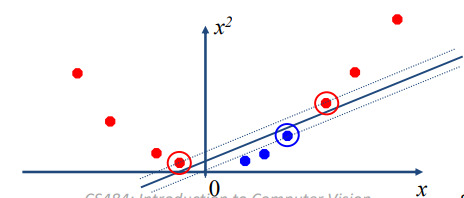
\includegraphics[width=8cm]{q1_2.png}
    \caption{after kernel}
    \label{fig:Question1}
\end{figure}
After using kernel, we can seperate them. 



%%%%%%%%%%%%%%%%%%%%%%%%%%%%%%%%%%%

\pagebreak
\paragraph{Q2:} In machine learning, what are bias and variance? When we evaluate a classifier, what are overfitting and underfitting, and how do these relate to bias and variance?

%%%%%%%%%%%%%%%%%%%%%%%%%%%%%%%%%%%
\paragraph{A2:} Bias is the difference between the expected prediction of our model and the correct value. And variance is the amount that the estimate of the target function will chage if different training data was used. Underfitting is when model is too "simple" to represent all the relevant class characteristics. When we do underfitting, we get high bias and low variance like left figure. It also means high training error and high test error. Overfitting is when model is too "complex" and fits irrelevant characteristic (like noise) in the data. When we do overfitting, we get low bias but high variance like right figure. It also means low training error and gigh test error.

\begin{figure}[!h]
    \centering
    \subfigure[]{
    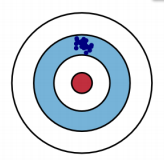
\includegraphics[width=4cm]{q2_1.png}
    }
    \subfigure[]{
    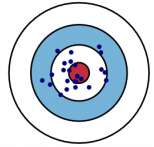
\includegraphics[width=4cm]{q2_2.png}
    }
    \caption{Underfitting and Overfiiting}
    \label{fig:Question2}
\end{figure}


%%%%%%%%%%%%%%%%%%%%%%%%%%%%%%%%%%%

% Please leave the pagebreak
\pagebreak
\paragraph{Q3:} Suppose we are creating a visual word dictionary using SIFT and $k$-means clustering for a scene recognition algorithm. Examining the SIFT features generated from our training database, we see that many are almost equidistant from two or more visual words. Why might this affect classification accuracy?

Given the situation, describe \emph{two} methods to improve classification accuracy, and explain why they would help.

%%%%%%%%%%%%%%%%%%%%%%%%%%%%%%%%%%%
\paragraph{A3:} Your answer here.



%%%%%%%%%%%%%%%%%%%%%%%%%%%%%%%%%%%

% Please leave the pagebreak
\pagebreak
\paragraph{Q4:} The way that the bag of words representation handles the spatial layout of visual information can be both an advantage and a disadvantage. Describe an example scenario for each of these cases, plus describe a modification or additional algorithm which can overcome the disadvantage. 

How might we evaluate whether bag of words is a good model?

%%%%%%%%%%%%%%%%%%%%%%%%%%%%%%%%%%%
\paragraph{A4:} Your answer here.



%%%%%%%%%%%%%%%%%%%%%%%%%%%%%%%%%%%

% If you really need extra space, uncomment here and use extra pages after the last question.
% Please refer here in your original answer. Thanks!
%\pagebreak
%\paragraph{AX.X Continued:} Your answer continued here.



\end{document}
